\begin{figure*}[ht]
    \centering
    \begin{minipage}[t]{0.32\textwidth}
        \centering
        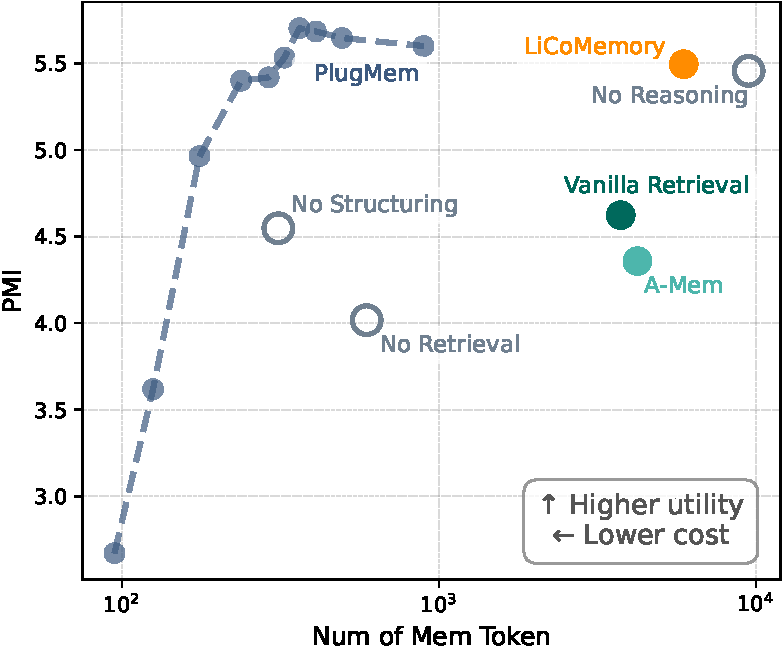
\includegraphics[width=\linewidth]{Figures/PMI_LME.pdf}
        {\small LongMemEval}
    \end{minipage}
    \hfill
    \begin{minipage}[t]{0.332\textwidth}
        \centering       
        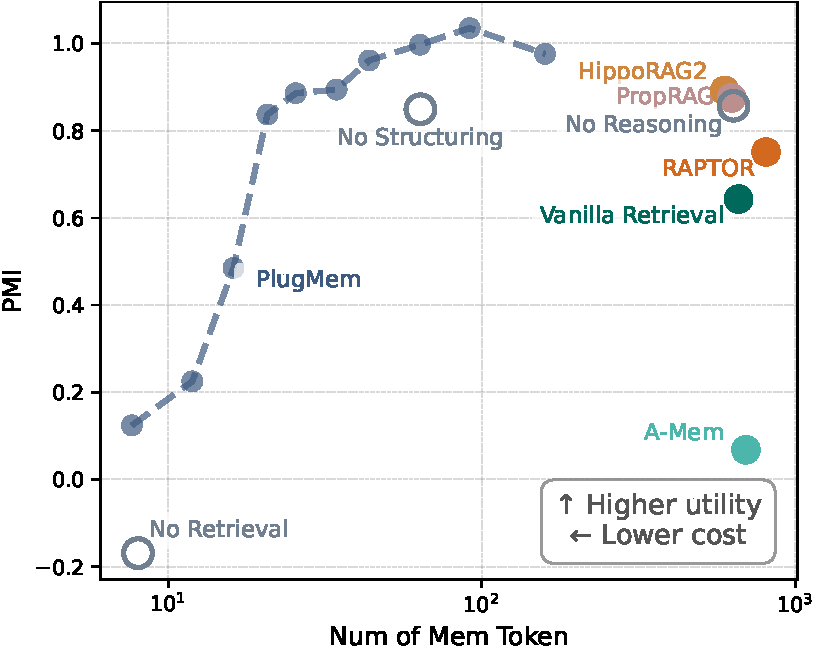
\includegraphics[width=\linewidth]{Figures/PMI_HotPotQA.pdf}
        {\small HotpotQA}
    \end{minipage}
    \hfill
    \begin{minipage}[t]{0.325\textwidth}
        \centering
        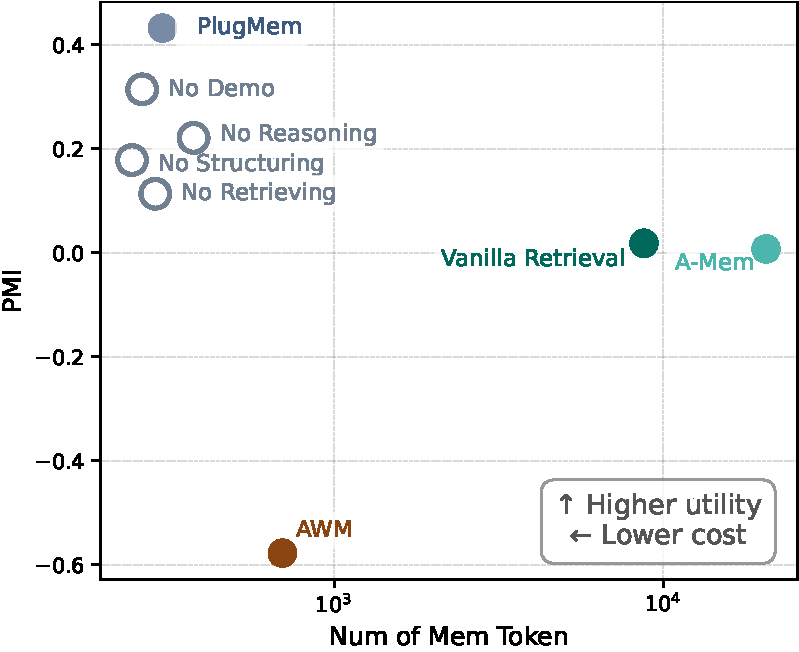
\includegraphics[width=\linewidth]{Figures/PMI_WebArena.pdf}
        {\small WebArena}
    \end{minipage}
    \caption{\label{fig:utility_cost}
    Utility–cost analysis across benchmarks. Each point represents a memory method, with the x-axis indicating agent-side memory cost (in tokens) and the y-axis indicating decision-relevant utility (in bits). The slope of the line connecting a point to the origin corresponds to information density (bit per token). Curves are obtained by sweeping the memory token budget on a randomly sampled subset of benchmark tasks, illustrating how memory utility initially increases with budget, then saturates, and may eventually decline as additional memory becomes counterproductive, for example by introducing noise or interference in decision-making. \textbf{\plugmem consistently achieves a more favorable utility–cost trade-off, dominating prior approaches by providing higher decision-relevant utility under smaller memory budgets across benchmarks.}
    }
\end{figure*}
